\section*{Figures}
\subsection*{Figure legends}

\noindent Figure 1. Global map of Large Marine Ecosystems (LMEs) and
high seas areas (ovals) showing the number of stock assessments present in the database for each area. \\

\noindent Figure 2. Taxonomic coverage of assessed marine species present in the
RAM Legacy database. The circle located near the middle of the circular
dendrogram represents kingdom Animalia and each subsequent branching
represents a different taxonomic group (Kingdom to Phylum to Class to
Order to Family to Genus to Species). The width of each line is
proportional to the square root of the number of assessments in the
database. The outermost lines represent species and the number of
lines is the number of assessments for each species. The names of
multi-assessment species are not repeated on the outermost portion of
the dendrogram but continue counter-clockwise from the first entry.
Note that branch lengths are chosen for graphical purposes and do not
convey phylogenetic distance.\\ 

\noindent Figure 3. Comparison of the taxonomic diversity of marine
species as provided by FishBase (top panel), the coverage of catch
data as provided by the Sea Around Us Project (SAUP) database (middle
panel) and the new RAM Legacy database (bottom panel). To facilitate the
identification of the taxonomic groups that are not presented in the catch
and assessment data, the FishBase branching pattern of the spoked dendrogram is
maintained to generate the other two dendrograms.\\ 

%\noindent Figure 4. Mean trophic level (obtained from FishBase) of the assessed species, grouped by their $B/B_{msy}$ and $U/U_{msy}$ ratios. \\

\noindent Figure 4. Orca plots showing the temporal coverage of (A)
catch/landings, (B) spawning stock biomass and (C) recruitment. The
temporal coverage for individual assessments is represented by thin
alternating black and grey horizontal lines in the main panels. Orca
plots are named because their distinctive shape is uncannily similar
to the individually-identifiable nicked and notched dorsal fins of
killer whales (orcas). Thick horizontal lines at the base of each main
panel represent the time periods which are present in 90\% (black) and
50\% (grey) of all series for that data type.  Subfigure histograms
contain the frequency of occurrence of the various timespans without
reference to time period. Solid and long-dash vertical lines within
the subfigures represent the median,
2.5\% and 97.5\% quantiles, respectively.\\

\noindent Figure 5. Current exploitation rate versus current biomass for 241
individual stocks. Exploitation is scaled relative to that which
should allow maximum sustainable yield ($U_{msy}$); biomass is scaled
relative to $B_{msy}$. Shades of grey indicate probability of occurrence as
revealed by a kernel density smooth function. Solid circles indicate
$B_{msy}$ and $U_{msy}$ that were obtained directly from assessments; open circles
indicate that they were estimated from surplus production models.\\ 

\noindent Figure 6. Current exploitation rate versus biomass for
individual stocks grouped by management unit. The panel labelled
``Atlantic'' comprises ICCAT and NAFO. Plot details as in
Figure 6.\\


\newpage
\subsection*{Figures}

\begin{figure}
\begin{center}
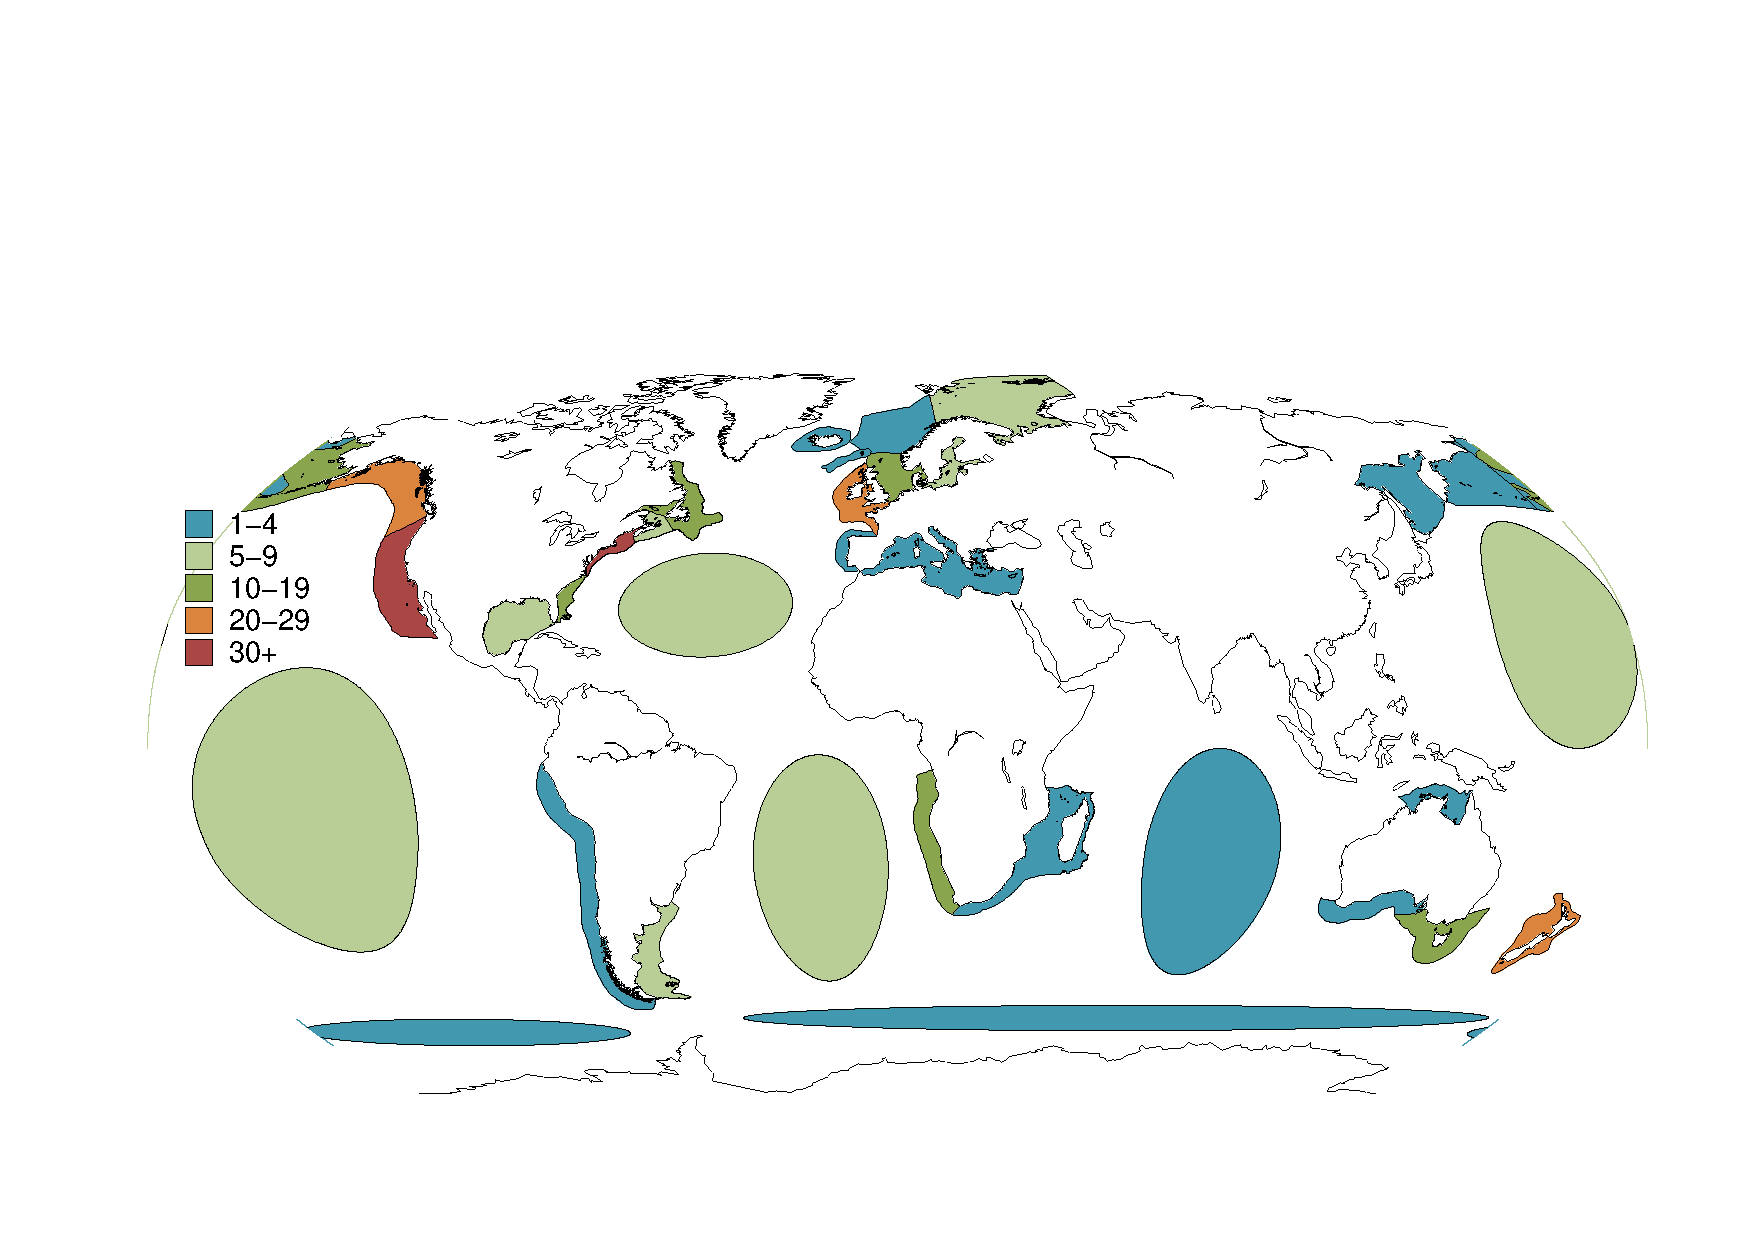
\includegraphics[width=\textwidth]{/home/srdbadmin/srdb/projects/fishandfisheries/GMT/stocks-byLME.pdf}
\end{center}
\caption{ }\label{fig:lmes}
\end{figure}

\begin{figure}
\begin{center}
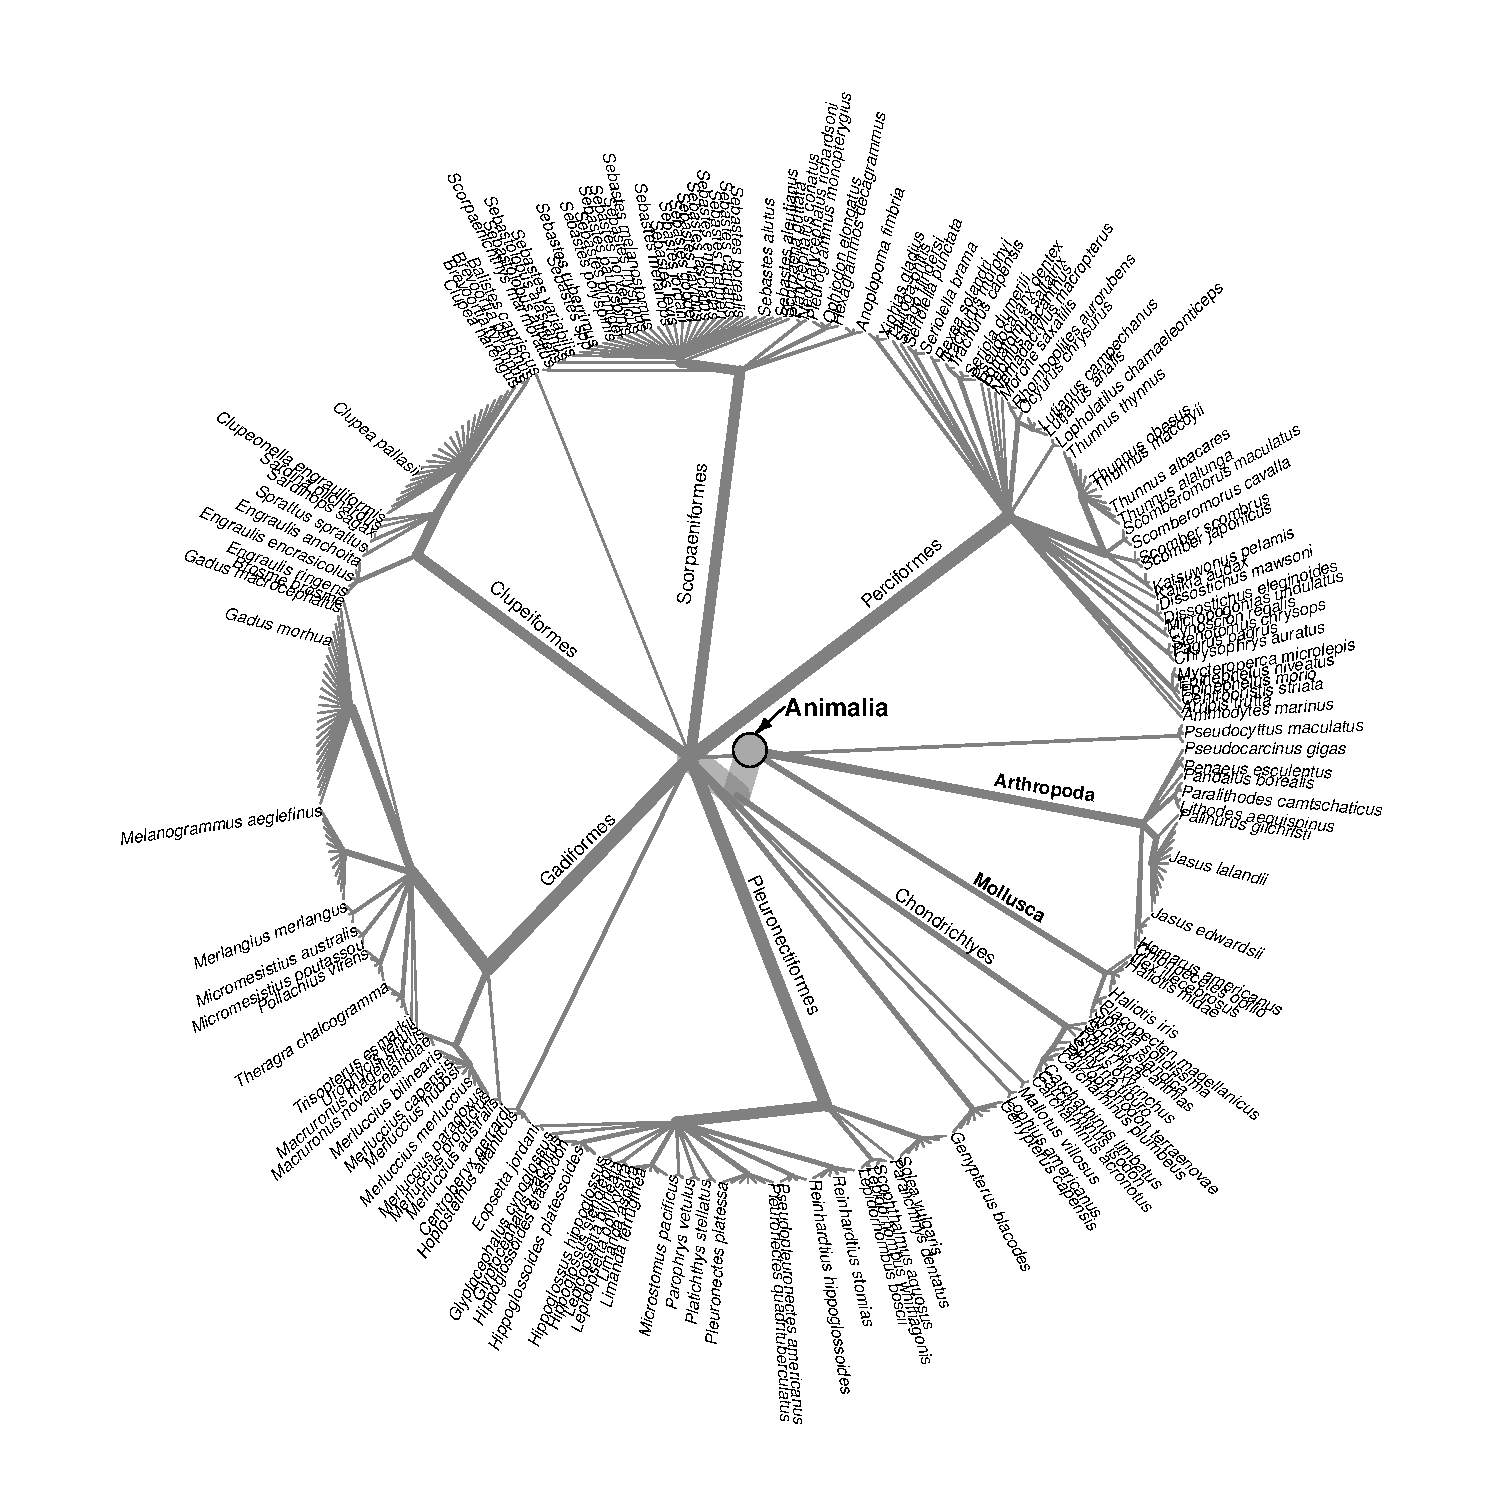
\includegraphics[width=7.5in]{/home/srdbadmin/srdb/projects/fishandfisheries/R/srdb-by-assessment.pdf} %taxonomic_coverage_byLME.pdf}
\end{center}
\caption{ }\label{fig:taxo:srdb}
\end{figure}


\begin{figure}
\begin{center}
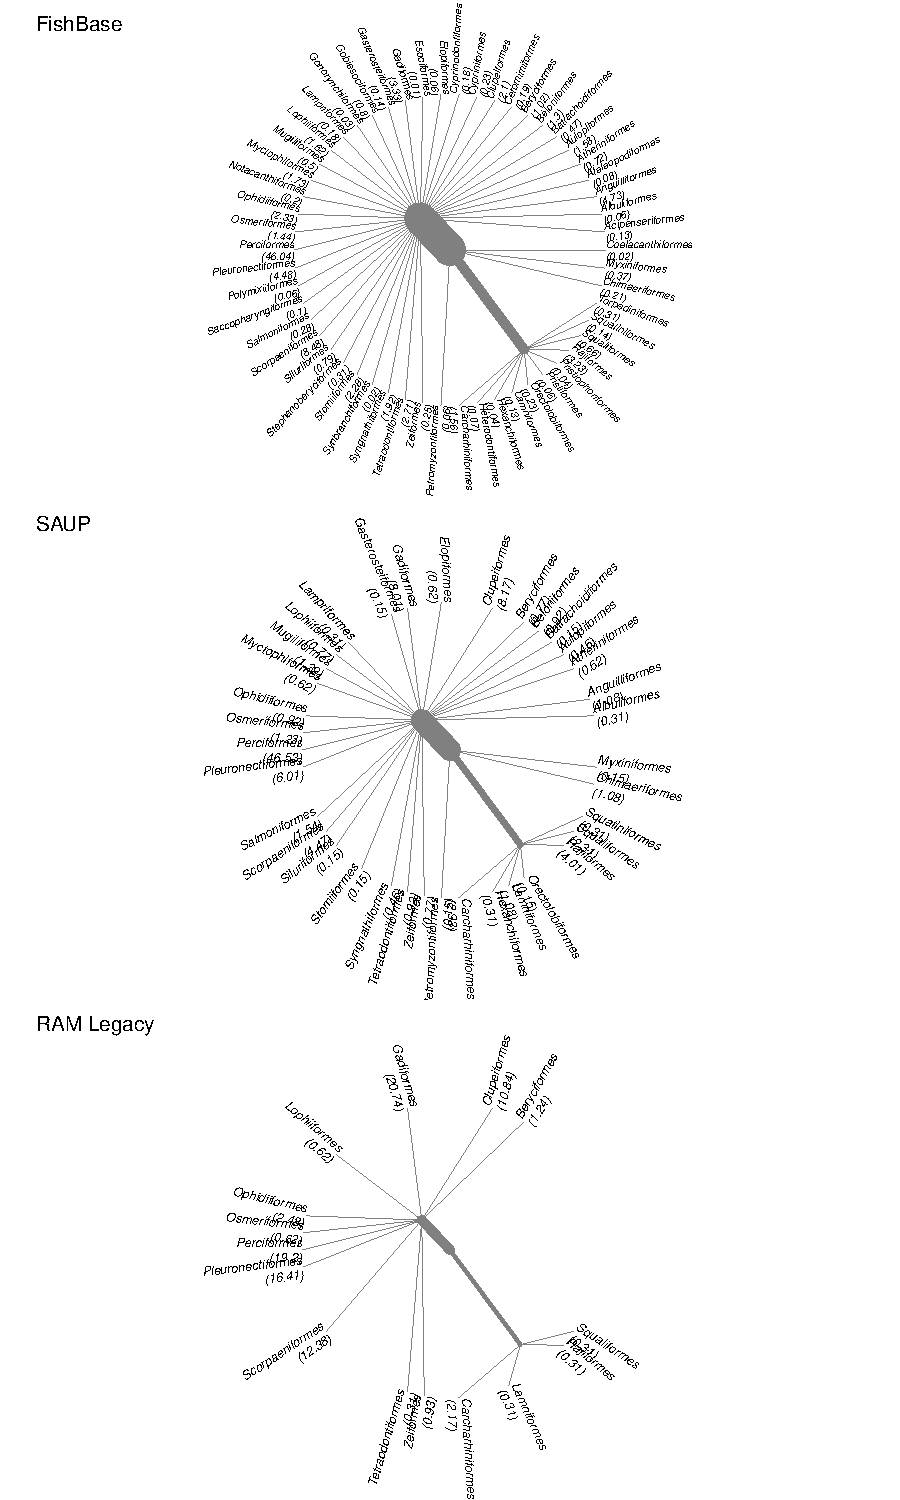
\includegraphics[height=9.5in]{/home/srdbadmin/srdb/projects/fishandfisheries/R/three_panel_phylo.pdf} % fishbase_saup_two_panel_phylo.pdf}
\end{center}
\caption{ }\label{fig:taxo:threepanel}
\end{figure}

%\begin{figure}
%\begin{center}
%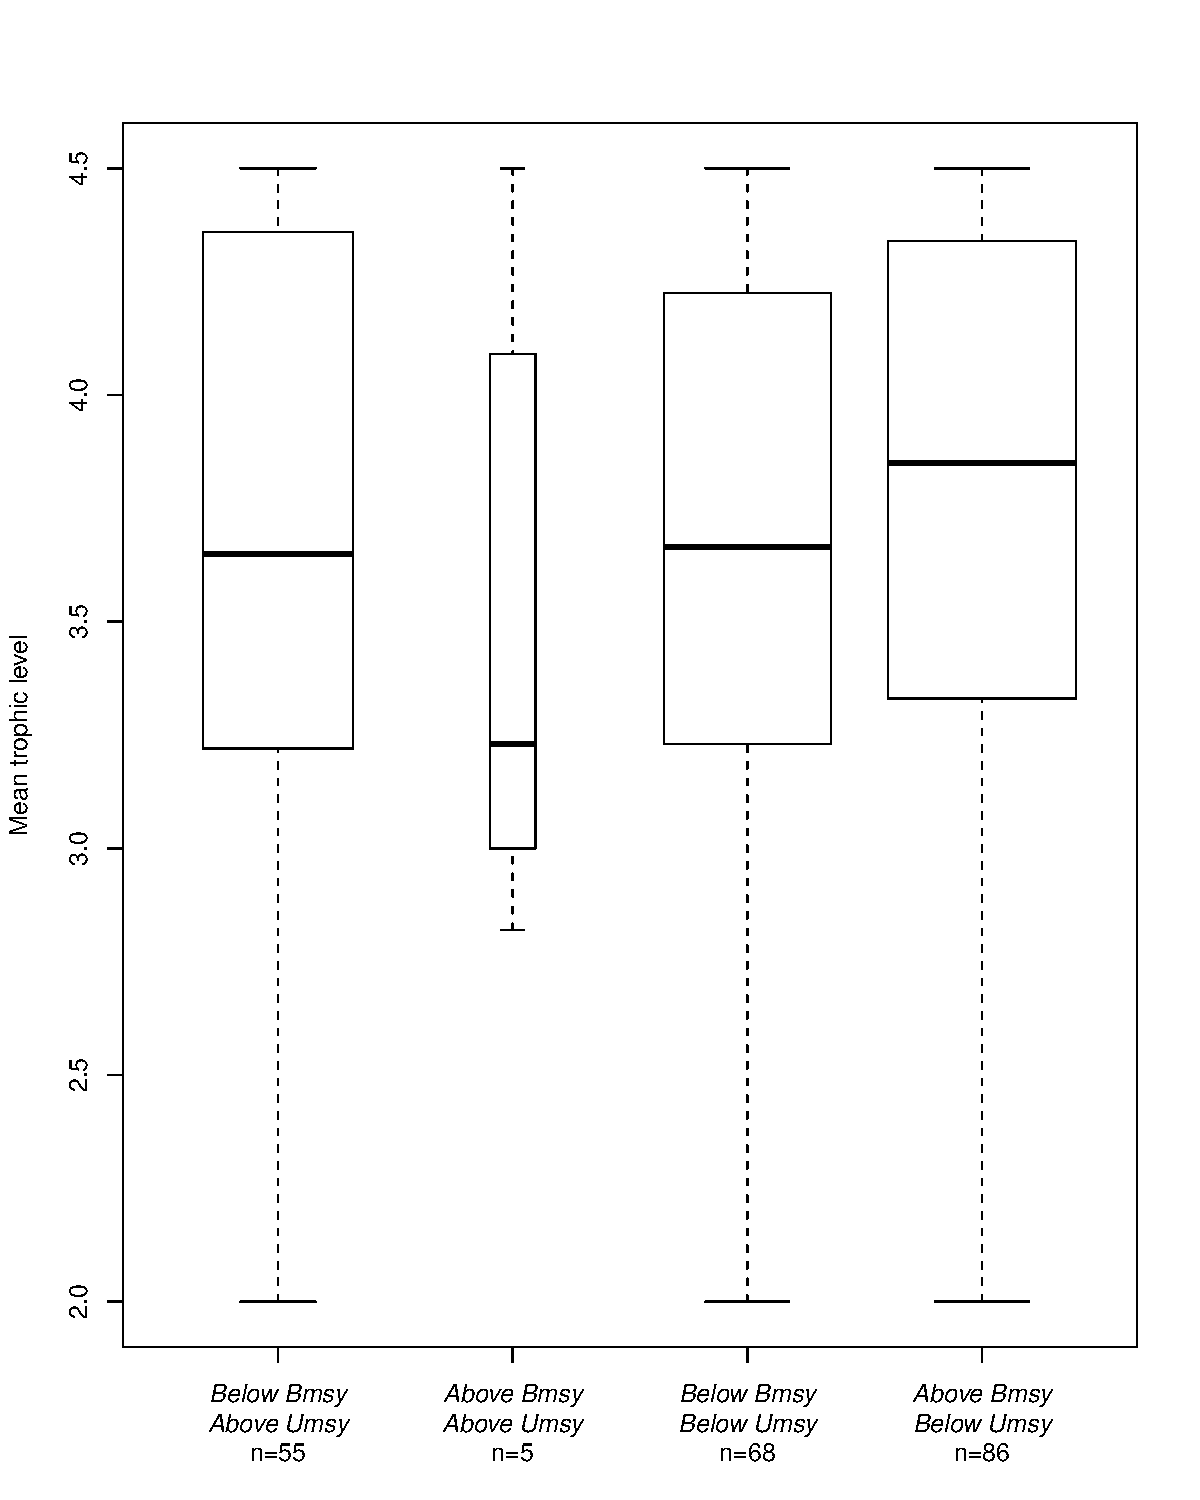
\includegraphics[width=15cm]{/home/srdbadmin/srdb/projects/fishandfisheries/R/TL-quadrant-srdb.pdf}
%\end{center}
%\caption{ }\label{fig:TL}
%\end{figure}

\begin{landscape}

\begin{figure}
\begin{center}
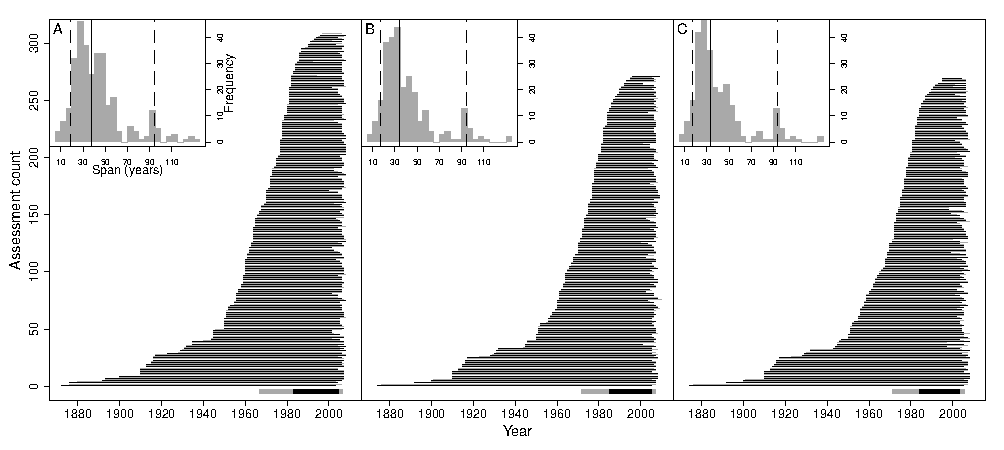
\includegraphics[width=8in]{/home/srdbadmin/srdb/projects/fishandfisheries/R/orca_plot_v2.pdf}
\end{center}
\caption{ }\label{fig:orca}
\end{figure}
\end{landscape}

\begin{figure}
\begin{center}
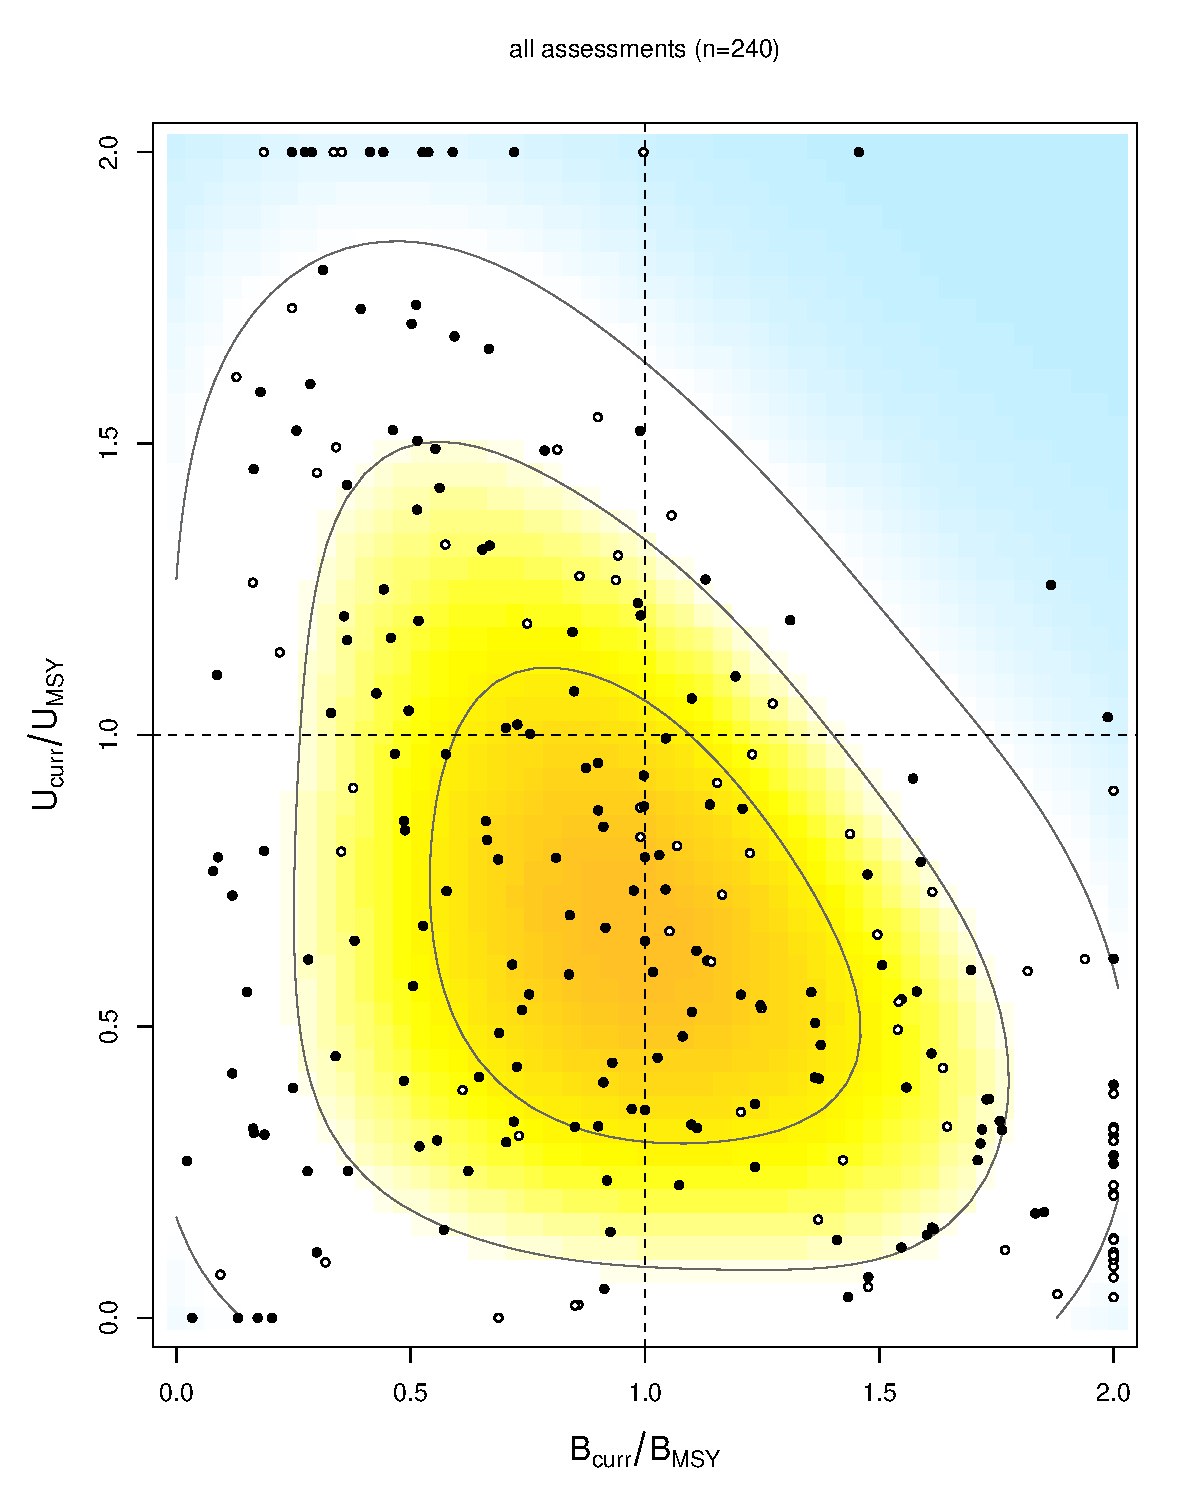
\includegraphics[width=15cm]{/home/srdbadmin/srdb/projects/fishandfisheries/R/friedegg-single.pdf}
\end{center}
\caption{ }\label{fig:friedegg}
\end{figure}

\begin{figure}
\begin{center}
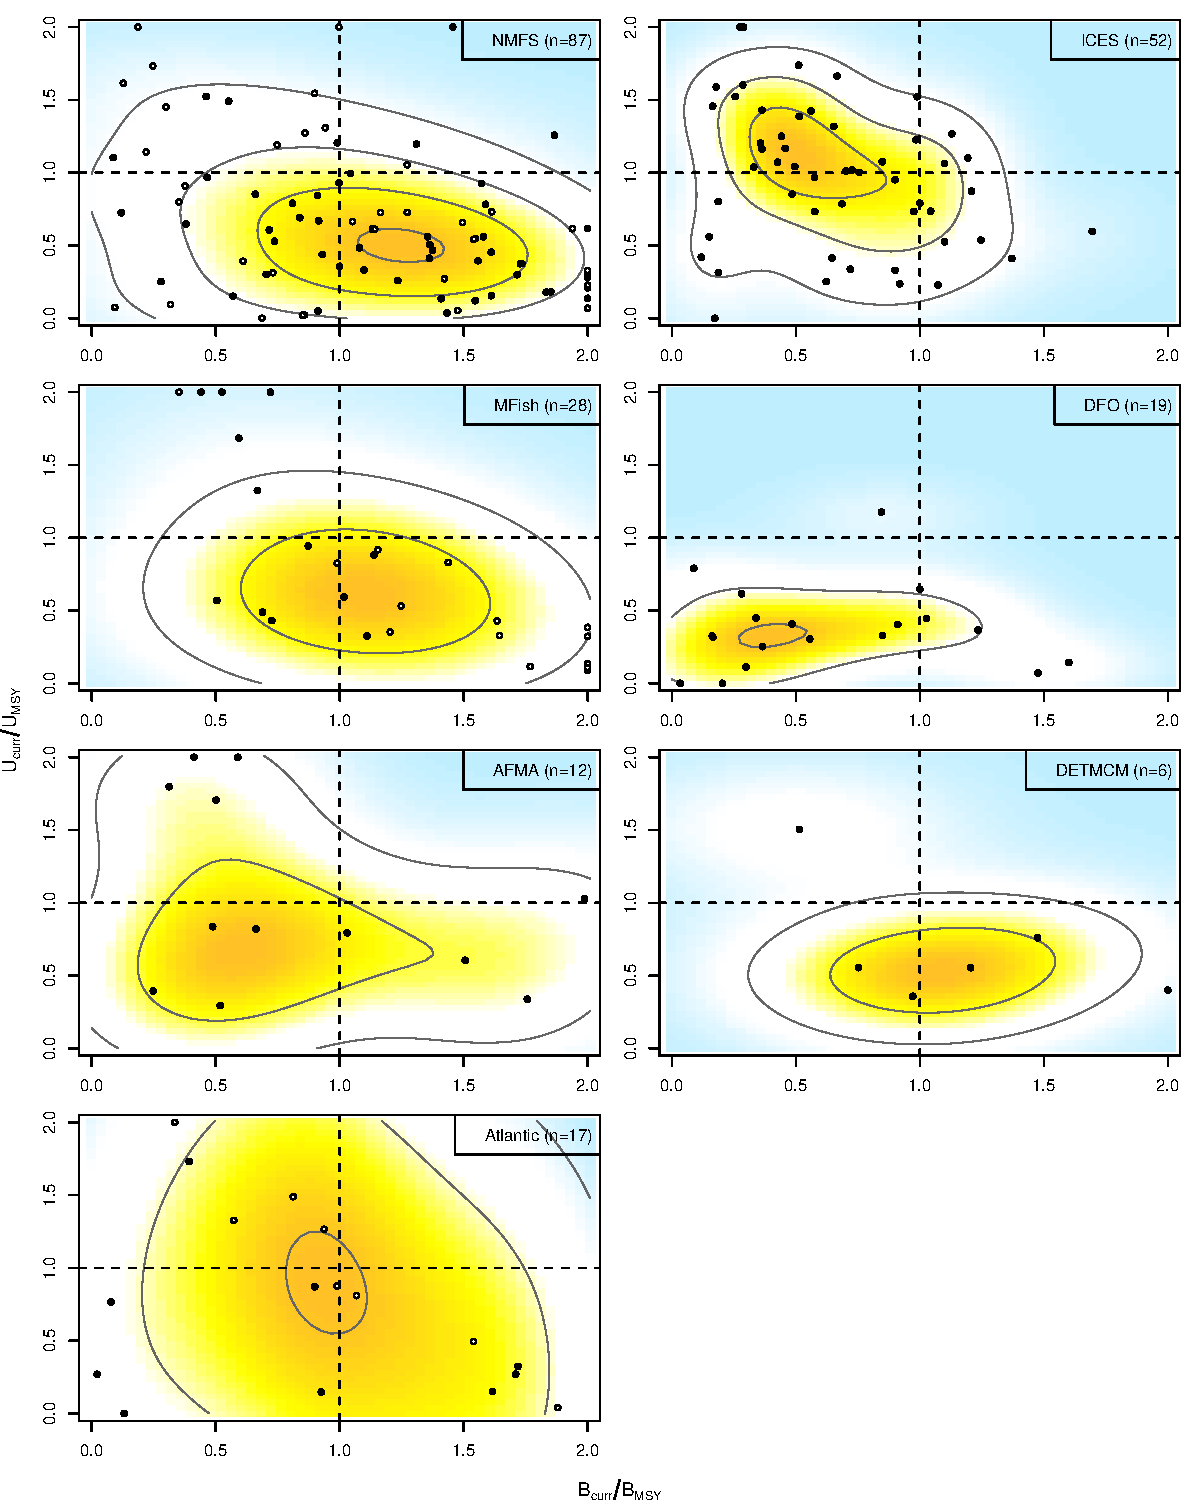
\includegraphics[width=15cm]{/home/srdbadmin/srdb/projects/fishandfisheries/R/friedegg-by-mgmt.pdf}
\end{center}
\caption{ }\label{fig:friedeggmgmt}
\end{figure}

